\documentclass{article}

\usepackage{arxiv}
\usepackage{markdown}
\usepackage{amsmath, xparse}
\usepackage[utf8]{inputenc} % allow utf-8 input
\usepackage[T1]{fontenc}    % use 8-bit T1 fonts
\usepackage{hyperref}       % hyperlinks
\usepackage{url}            % simple URL typesetting
\usepackage{booktabs}       % professional-quality tables
\usepackage{amsfonts}       % blackboard math symbols
\usepackage{nicefrac}       % compact symbols for 1/2, etc.
\usepackage{microtype}      % microtypography
\usepackage{cleveref}       % smart cross-referencing
\usepackage{lipsum}         % Can be removed after putting your text content
\usepackage{graphicx}
\usepackage{natbib}
\usepackage{doi}

\usepackage{titlesec}

\setcounter{secnumdepth}{4}

% \title{Interpretation \emph{arxiv} style}
\title{Electronic Color Code Interpretation for Through Hole Resistor}

% Here you can change the date presented in the paper title
%\date{September 9, 1985}
% Or remove it
%\date{}

%\author{ \href{https://orcid.org/0000-0000-0000-0000}{
\includegraphics[scale=0.06]{orcid.pdf}\hspace{1mm}David S.~Hippocampus}\thanks{Use footnote for providing further information about author (webpage, alternative address)---\emph{not} for acknowledging funding agencies.}
\author{{YUE-ER, HSU} \\
	Department of Electrical Engineering\\
	National Cheng Kung University\\
	No. 1 University Road, Tainan City 70101, Taiwan (R.O.C.) \\
	\texttt{e24074724@mail.ncku.edu.tw} \\
	%% examples of more authors
	%% \And
	%% \href{https://orcid.org/0000-0000-0000-0000}{
\includegraphics[scale=0.06]{orcid.pdf}\hspace{1mm}Elias D.~Striatum} \\
	%% Department of Electrical Engineering\\
	%% Mount-Sheikh University\\
	%% Santa Narimana, Levand \\
	%% \texttt{stariate@ee.mount-sheikh.edu} \\
	%% \AND
	%% Coauthor \\
	%% Affiliation \\
	%% Address \\
	%% \texttt{email} \\
	%% \And
	%% Coauthor \\
	%% Affiliation \\
	%% Address \\
	%% \texttt{email} \\
	%% \And
	%% Coauthor \\
	%% Affiliation \\
	%% Address \\
	%% \texttt{email} \\
}

% Uncomment to override  the `A preprint' in the header
%\renewcommand{\headeright}{Technical Report}
%\renewcommand{\undertitle}{Technical Report}
%\renewcommand{\shorttitle}{\textit{arXiv} Template}
\renewcommand{\shorttitle}{Electronic Color Code Interpretation for Through Hole Resistor}

%%% Add PDF metadata to help others organize their library
%%% Once the PDF is generated, you can check the metadata with
%%% $ pdfinfo template.pdf
\hypersetup{
pdftitle={A template for the arxiv style},
pdfsubject={q-bio.NC, q-bio.QM},
pdfauthor={David S.~Hippocampus, Elias D.~Striatum},
pdfkeywords={First keyword, Second keyword, More},
}

\begin{document}
\maketitle

\begin{abstract}
%%	\lipsum[1]
Use machine learning and computer vision methods to practice the resistance value identification of color-coded resistors, and improve the accuracy of interpretation through Root-Polynomial Regression method color preprocessing correction and YOLOV5 object detection model. Comparing the difference in accuracy using openCV and ML models, the goal is to support color casts and lower resolution resistive images. In addition, in terms of model training, a self-made data set is planned to be used for migration training to improve software performance. It is expected to be packaged into a progressive web application for ordinary users to perform resistance identification operations in field fields such as laboratories through smartphones with camera lenses.
\end{abstract}


% keywords can be removed
\keywords{First keyword \and Second keyword \and More}


\section{Introduction}
%\lipsum[2]
%\lipsum[3]

\subsection{Research purposes}

\begin{itemize}
	\item Train a machine learning model that detects color-coded resistance
	\item Capture the resistor image and correct the pattern
	\item Color correction of resistive image using algorithm
	\item Capture the color ring of the color-coded resistor and calibrate its value
	\item Use the image classification task to discriminate the resistance value and compare the difference in accuracy
	\item Build a PWA capable of edge computing
\end{itemize}

\subsection{Background brief}
Many electronic parts use color-coded rings to represent values, including but not limited to resistors, inductors, etc. These are again dominated by Through Hole Resistors. It is a time-consuming task to manually select a specific value among many scattered solid parts, and its accuracy is not good. Although the current production line has an automatic identification system, its environment is often relatively simple. A monochrome background and a stable light source are required, which cannot be applied by analogy. If an application program mounted on a smartphone can be built, the problem of selecting discrete components in a general laboratory environment can be solved, and a fully automatic or semi-automatic material selection system can be achieved.

\subsection{Literature Discussion}
There are many existing solutions for resistance color code identification, but most of them are achieved with openCV, which can only identify a single object in the screen, and is limited by the angle, position, and ambient light source of the object, and its accuracy cannot be achieved in the real environment. The image captured by the real environment lens has the following problems: (1) underexposure and overexposure caused by ambient light sources or camera settings, (2) reflections caused by ambient light sources or resistive materials, (3) ) non-solid color background, (4) similar peripheral circuits or components, (5) too low resolution or too small components, (7) blur due to motion, (8) color cast.
In order to deal with the above problems and build a resistance identification system that is closer to the real environment, in this topic, we will compare the accuracy and performance differences of resistance color code identification using openCV technology and YOLO technology.

\subsection{problem statement}
Develop an application program, which can be mounted on a smart phone with a lens (supports android and ios platforms), and can provide users to identify the resistance value of the color-coded resistor. and achieve the following functions
1. Mark all identified resistors in the scene
2. Frame the resistance range
3. Mark all the list of resistors in the scene
4. Supports the identification of any angle
5. With real-time identification function
6. Great tolerance for ambient light sources
7. Complex backgrounds still work

The sample input and output screens are as follows:

\begin{figure}
	\centering
	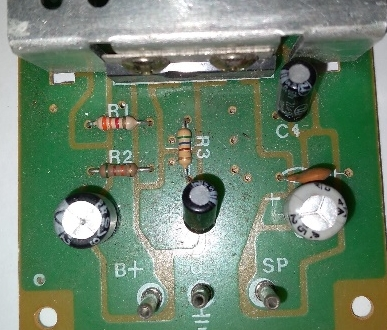
\includegraphics[width=0.7\linewidth]{doc1.jpg}
	\caption{Sample figure caption.}
	\label{fig:doc1}
\end{figure}

\begin{figure}
	\centering
	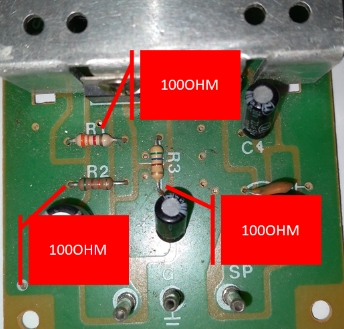
\includegraphics[width=0.7\linewidth]{doc2.jpg}
	\caption{Sample figure caption.}
	\label{fig:doc2}
\end{figure}

Input screen example (not limited to identifying resistors on PCB, should support resistor object identification on any background)
Example of output screen (frame selection of resistance objects, read the value according to its color code, superimpose and display it on the screen)

\subsection{This article solves the problem}
The expected software flow is (in order): (1) user input of dynamic images with or without resistors, (2) image preprocessing, (3) machine learning model prediction and box selection of resistive objects, (4) resistive objects Image normalization, (5) data interpretation, (6) composite output image, (7) output composite image with resistance judgment value and related information to users
Among them, the above sub-projects 2-5 will be implemented by computer vision method and machine learning method respectively, and the differences will be compared.
4. Method
In an environment with GeForce RTX 2080 TI or similar computing power, using python language, using PyTorch as the framework, and adopting the YOLOV5 identification system, the transfer training of the identification model is carried out. The training data set is recorded on the camera using a conventional smartphone, and then generated by manual and automatic marking after the image processing. In addition, in the data collection stage, in order to improve the accuracy, a verification data set will be generated by a crawler to verify the model. .
For the part of image preprocessing, including color and angle correction, it is carried out with openCV, and the actual image situation is analyzed in the process, and the best algorithm or model is tested and experimented.

\subsection{Where innovation lies}
According to the specification of color code marking, different manufacturers will make different series of resistors. We cannot solve the problem of color code resistance identification by classification problem. We use an end-to-end solution, which is similar to the example method of image to latex. , a RNN is connected in series behind the CNN, and the focus method is used to train the model to learn to output the direct resistance value. In this way, our results can cover all possible resistance values, rather than being limited to discrete components that can be purchased at local electronic materials stores.

\subsection{Summary Statement of Implementation Results}

\begin{figure}
	\centering
	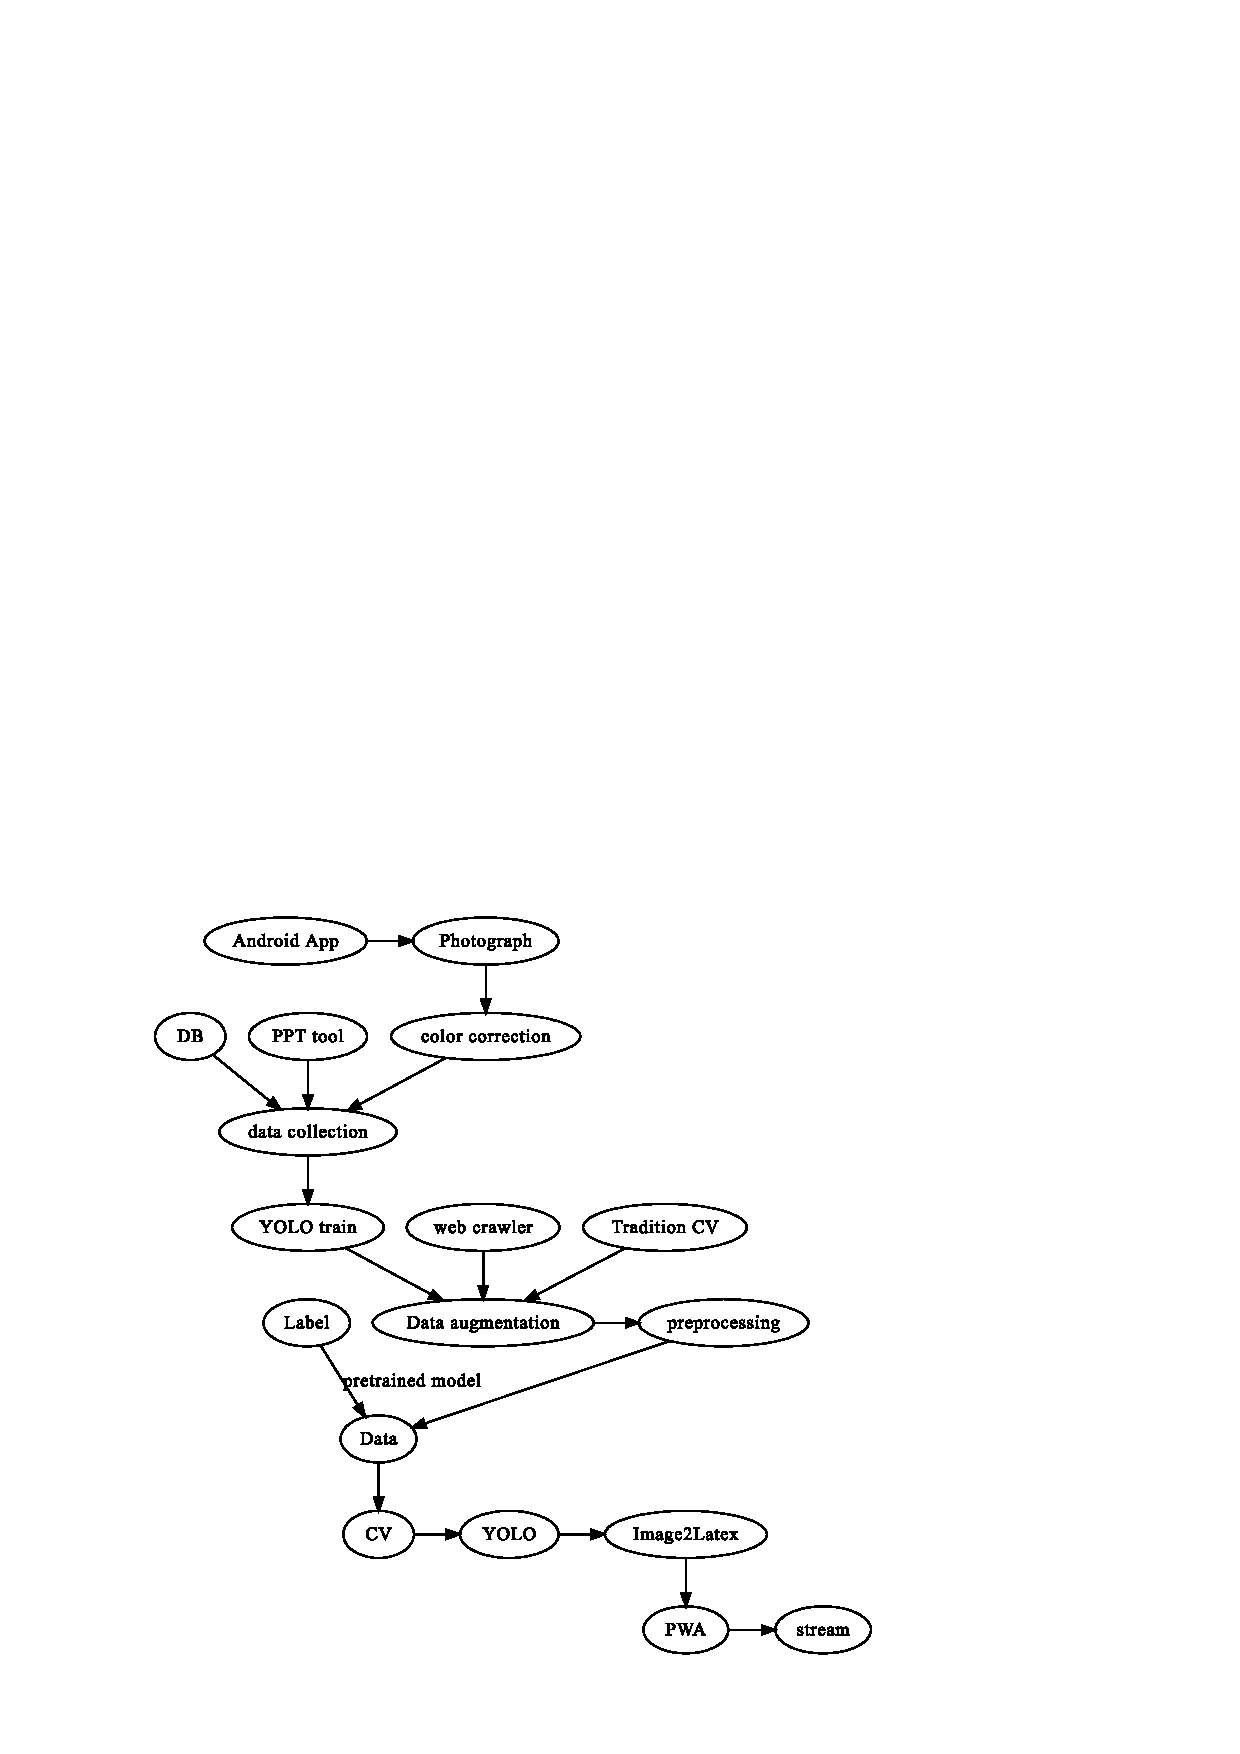
\includegraphics[width=0.7\linewidth]{ppp10.pdf}
	\caption{Sample figure caption.}
	\label{fig:ppp10}
\end{figure}

\section{Principle Analysis and System Design}
\subsection{Principle Analysis}

\subsubsection{Resistor Color Code Rules}
The color code of discrete resistance components represents its value. We only discuss the perforation elements without discussing the chip components. The color code ring will have the following colors: black, brown, red, orange, yellow, green, blue, purple, gray, white, gold, silver, respectively represent numbers 1 to 9 and errors, respectively. Discrete resistance components have a four -color ring or five -color ring, which represents different resistance accuracy, and its reading value method is similar. Taking an instance of the four -color ring as an example, the first two representatives of the scientific marks, the third digit is the second part, and the fourth place is only gold or silver, which represents the error of 5 or 10 percentage.

\subsubsection{image preprocessing}

%(A) Introduction \\In many image recognition situations, it is necessary %to know whether an image is head up. In this project, we are trying to %solve a real world problem.

\paragraph{Problem statement}
Consider a camera and a color code resistor, let a user hold the camera to take an image of the color code resistor, where the color code resistor is placed in any direction.
Try to use an algorithm to determine whether the resistor is “horizontally placed”.

Picture 1: Many resistors in different directions

Picture 2: Color coded resistors defined as “horizontally placed”

\begin{figure}
	\centering
	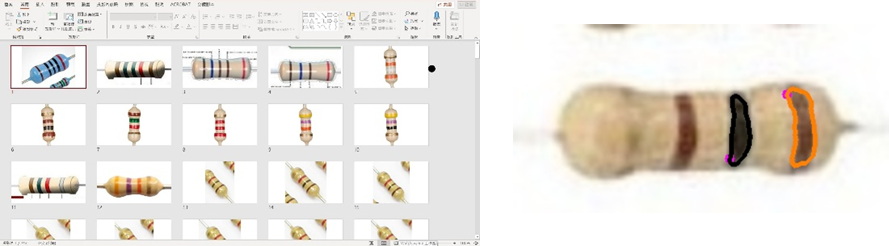
\includegraphics[width=0.7\linewidth]{Wr4nVKT.png}
	\caption{Sample figure caption.}
	\label{fig:wr4nvkt}
\end{figure}

\paragraph{Definition}

We have just derived the Radon transform of the function f(x,y). So

$p_\vartheta(r)=\int_{-\infty}^{\infty}vf(rcos(\theta)-zsin(\theta),\ rsin(\theta)+zcos(\theta))\ dz$

where $p_\vartheta$ is the Radon transform of f(x,y).\citep{githubGitHubGpeyrenumericaltours}

figure 3.: Geometric interpretation

\begin{figure}
	\centering
	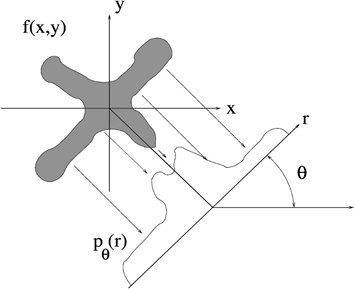
\includegraphics[width=0.7\linewidth]{NwQ7eeG.png}
	\caption{Sample figure caption.}
	\label{fig:NwQ7eeG}
\end{figure}

Notice that the projection corresponding to $r=0$ passes through the point $(x,y)=(0,0)$.Also note that theoretically, projections are only required for $\vartheta \in [0°, 180°)$. It does not matter which direction you integrate from along the z-axis. $p_\vartheta(r)=p_\vartheta+180(r)$ for $\vartheta \in [0°, 180°)$. As long as you have collected the projections for $\vartheta \in [0°, 180°)$, further measurements will produce only redundant information. In practice however, taking measurements over [0°,360°) could be advantageous in terms of better signal to noise ratio. Also in practice, the measurement is discretized so if you place your detectors so none of them are exactly 180° from each other but have a slight offset, you can collect information from a larger amount of unique data points. So in practice scanners do perform measurements for angles larger than 180°.\citep{projectrheaECE637Tomographic}

\paragraph{Relation with Fourier transform}

By definition


\begin{eqnarray}    \label{eq}
	{P_{\theta}(\rho)}&=&CTFT\{p_{\theta}(r)\}  \nonumber    \\
	~&=&\int_{-\infty}^{\infty}p_{\theta}(r)e^{-j2\pi\rho r}\ dr \nonumber    \\
	~&=&\int_{-\infty}^{\infty}[\int_{-\infty}^{\infty}f(A_{\theta}\begin{bmatrix}
		r \\
		z \\
	\end{bmatrix})dz]e^{-j2\pi\rho r}\ dr \nonumber    \\
	~&=&\int_{-\infty}^{\infty}\int_{-\infty}^{\infty}f(A_{\theta}\begin{bmatrix}
		r \\
		z \\
	\end{bmatrix})e^{-j2\pi\rho r}\ dz\ dr
\end{eqnarray}

Next we make the following change of variables

$\begin{bmatrix}
	r \\
	z \\
\end{bmatrix}=A_{-\theta}\begin{bmatrix}
	x \\
	y \\
\end{bmatrix}$

where the Jacobian is $|A_{-\theta}|=1$

since

\begin{eqnarray}    \label{eq2}
	{|\frac{\partial(r,\ z)}{\partial(x,\ y)}|}&=&det\begin{bmatrix}
		\frac{\partial r}{\partial x} & \frac{\partial r}{\partial y} \\
		\frac{\partial z}{\partial x} & \frac{\partial z}{\partial y} \\
	\end{bmatrix} \nonumber    \\
	~&=&det\begin{bmatrix}
		\frac{\partial (xcos(\theta)+ysin(\theta))}{\partial x} & \frac{\partial (xcos(\theta)+ysin(\theta))}{\partial y} \\
		\frac{\partial (-xsin(\theta)+ycos(\theta))}{\partial x} & \frac{\partial (-xsin(\theta)+ycos(\theta))}{\partial y} \\
	\end{bmatrix} \nonumber    \\
	~&=&det\begin{bmatrix}
		cos\theta & sin\theta \\
		-sin\theta & cos\theta\\
	\end{bmatrix} \nonumber    \\
	~&=&cos^2\theta+sin^2\theta \nonumber    \\
	~&=&1
\end{eqnarray}

then

\begin{eqnarray}    \label{eq3}
	dr\ dz&=&|\frac{\partial(r,\ z)}{\partial(x,\ y)}|dx\ dy \nonumber    \\
	~&=&dx\ dy
\end{eqnarray}

plug in $r=xcos(\theta)+ysin(\theta)$

so we can get

\begin{eqnarray}    \label{eq4}
	P_{\theta}(\rho)&=&\int_{-\infty}^{\infty}\int_{-\infty}^{\infty}f(x,y)e^{-j2\pi\rho[xcos(\theta)+ysin(\theta)]}\ dx\ dy \nonumber    \\
	~&=&\int_{-\infty}^{\infty}\int_{-\infty}^{\infty}f(x,y)e^{-j2\pi[x\rho cos(\theta)+y\rho sin(\theta)]}\ dx\ dy \nonumber    \\
	~&=&F(\rho cos(\theta),\rho sin(\theta))
\end{eqnarray}

\begin{figure}
	\centering
	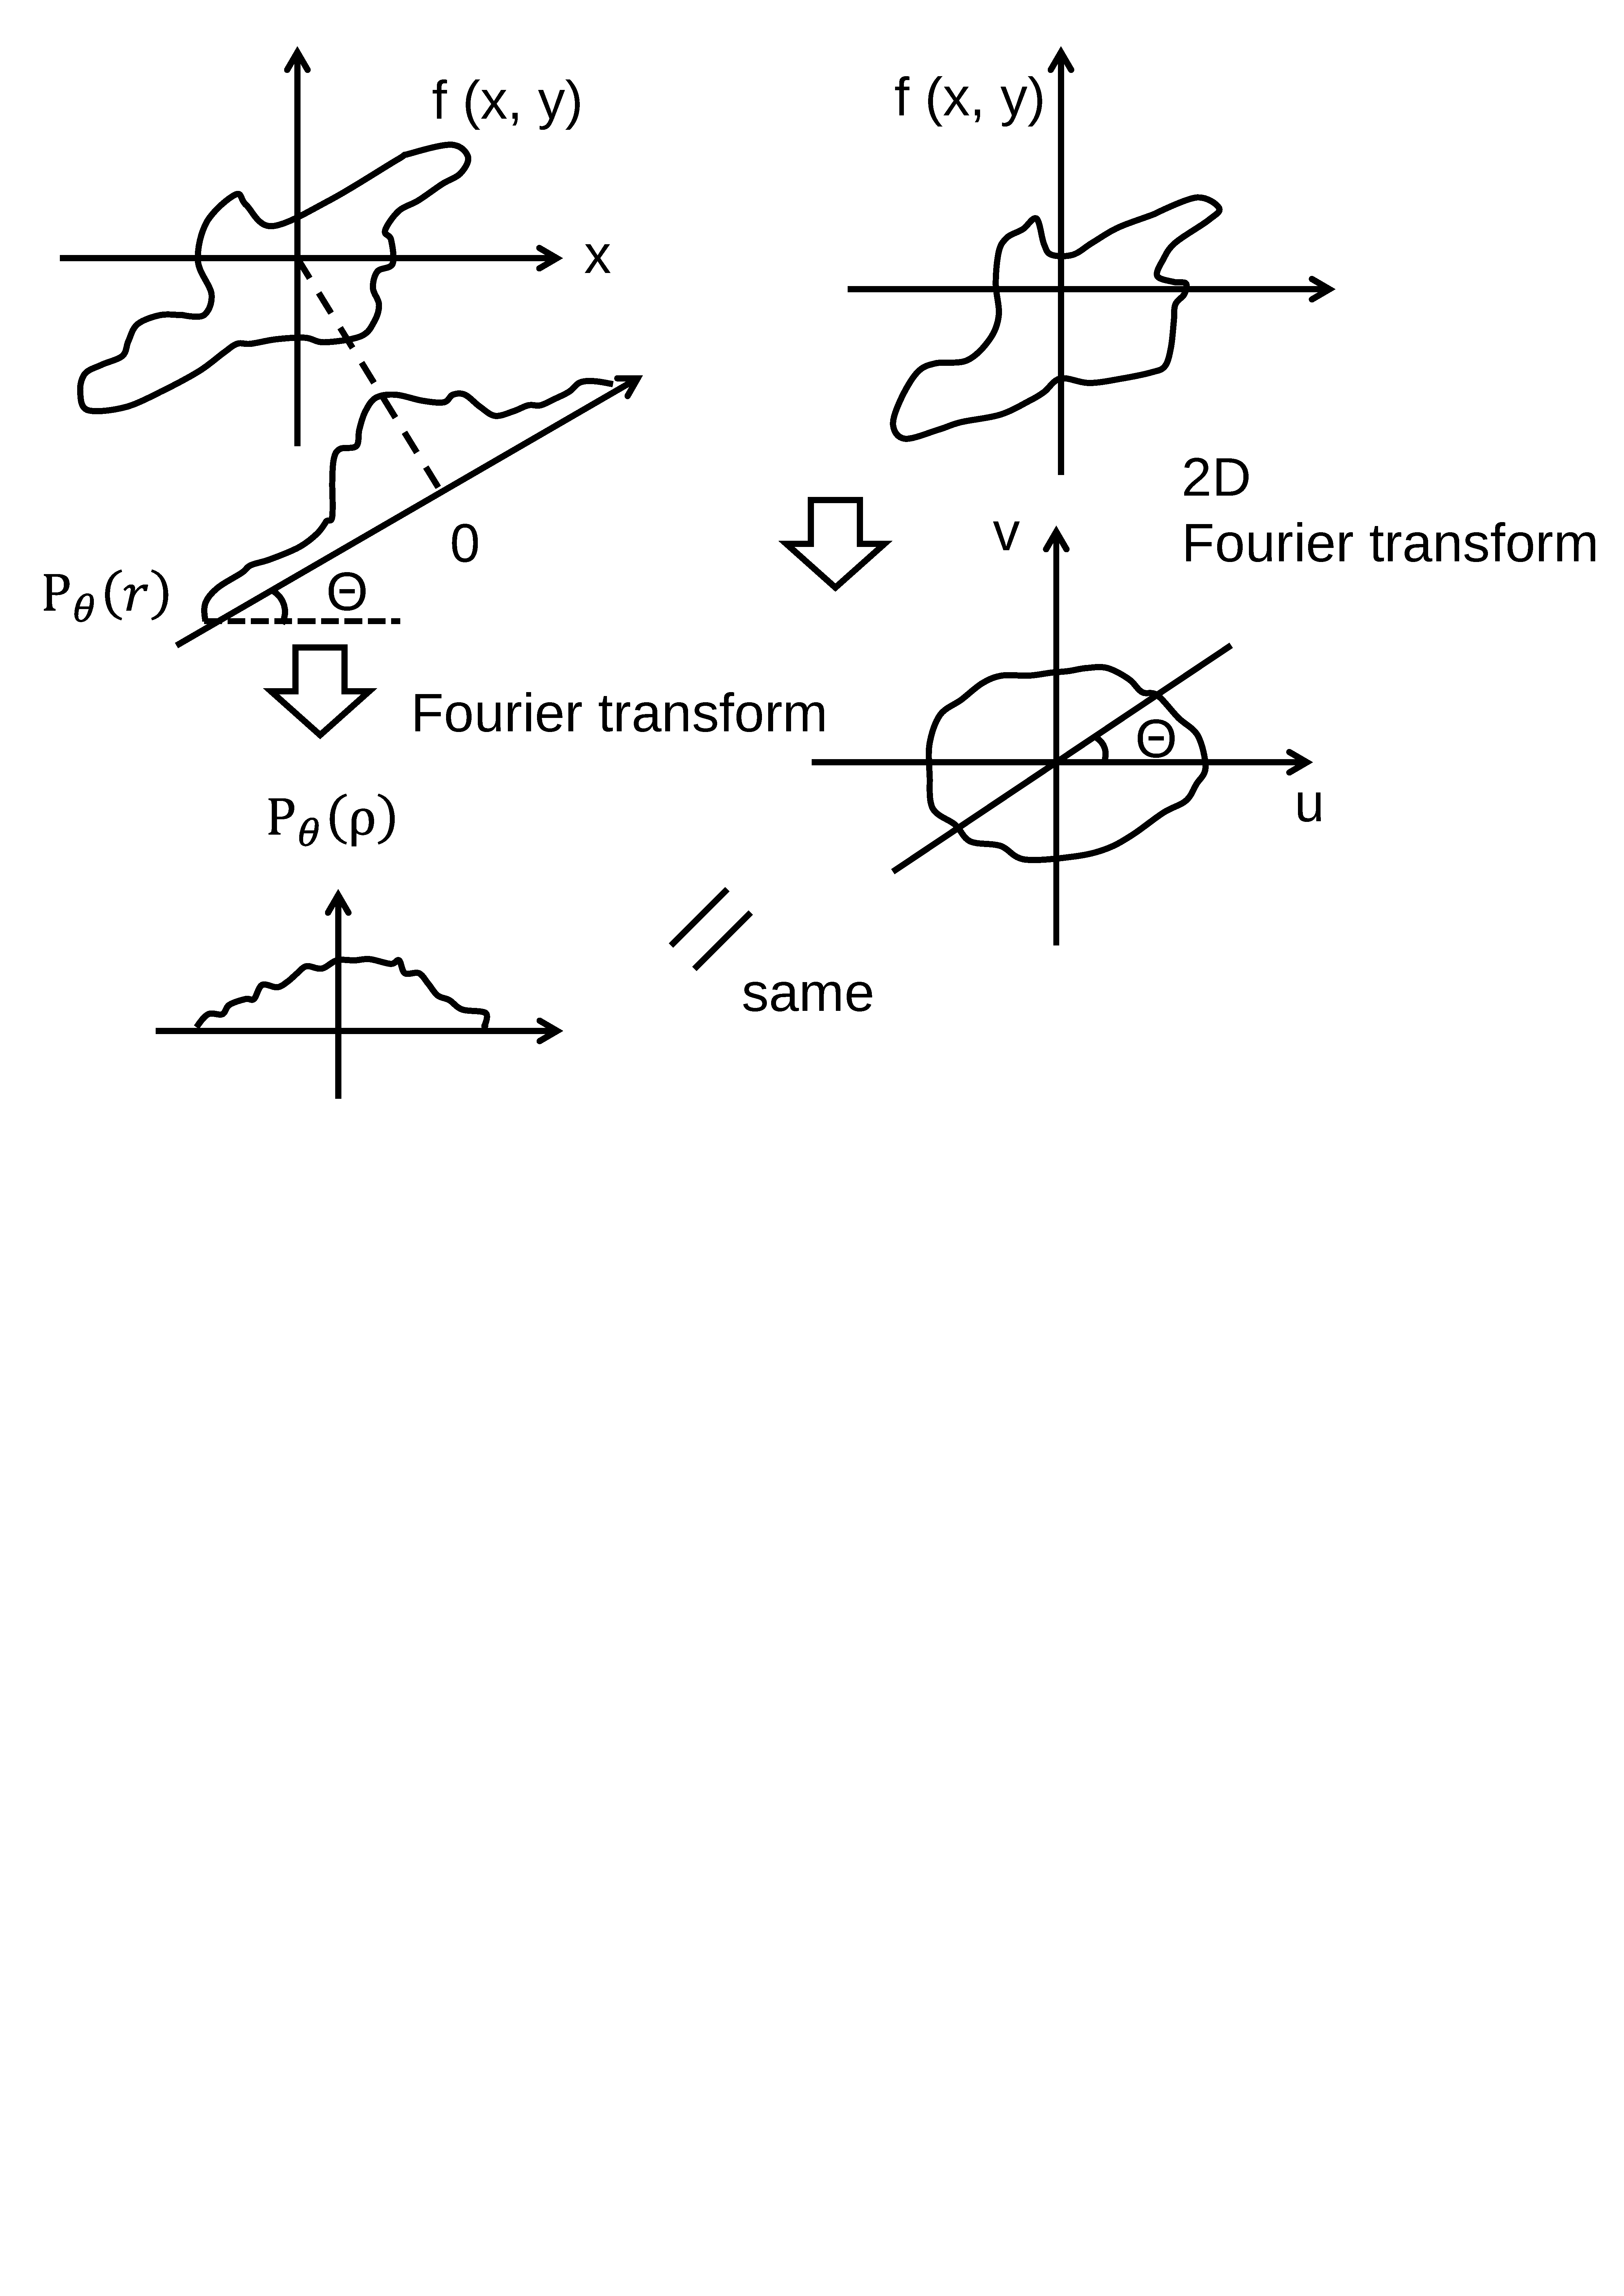
\includegraphics[width=0.7\linewidth]{p1.pdf}
	\caption{Sample figure caption.}
	\label{fig:p1svg}
\end{figure}

Although Fourier slice theorem allows us to reconstruct f(x,y),  practically it requires extremely large amount of data. Thus, convolution back projection is a preferred method to recover the picture. In conclusion, the radon function computes projections of an image matrix along specified directions.\citep{mathworksRadonTransform}

\paragraph{Implementation-Resistance Radon Matlab Code}

(a) Summary

Use matlab program to practice an image orientation corrector.
Especially used in the correction of the through hole color code resistance image.
The orientation angle of resistance pattern object placed at any angle is solved and corrected by radon transformation.

(b) Preface

This program is suitable for correcting the orientation of the color code resistance image
Consider an imaginary line through both metal wire connection point located at both ends of the resistor, define such line as "correct" orientation, and it must face the 90 degree direction of the Cartesian coordinate system.

(c) Function

The user needs to have a matlab program to execute this code.
The user can enter a picture of the resistor in this code. The picture is recommended to be taken with a camera. The position of the resistor must be in the center of the photo and the direction should be random.
After executing this program, you can see a orientation corrected resistance image and know the angle of the rotation.

(d) specifications

This program is only developed and tested under Windows operating system.

(1) Input specifications

%There is a string on line 13 in this code, that is where you need to modify.

1. Prepare a folder with many photos of resistors.
> The filename extension of photos must be JPG
2. Change the content of the preceding string to an absolute path to the folder.

A clean photo background is recommended.

(2) Sample input and test data

\begin{figure}
	\centering
	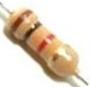
\includegraphics[width=0.7\linewidth]{e5hIvV0.jpg}
	\caption{Sample figure caption.}
	\label{fig:e5hIvV0jpg}
\end{figure}

(3) Output specifications

%There is a string on line 16 in this code, that is where you need to modify.

1. Prepare an empty folder.
2. Change the content of the preceding string to an absolute path to the folder.

You can get many images corrected by the program, the number of images is the same as the number of input files; that is, the program supports batch processing.

(4) Example output and explanation

\begin{figure}
	\centering
	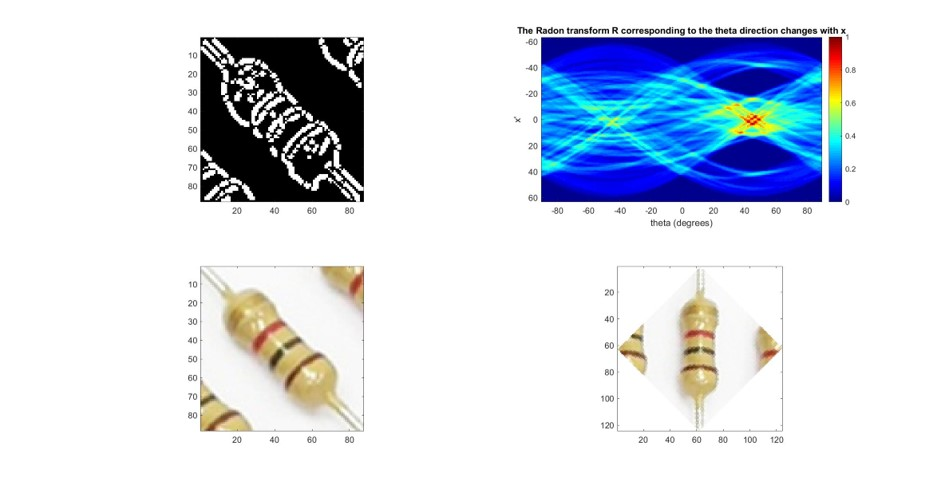
\includegraphics[width=0.7\linewidth]{DmQ3syQ.jpg}
	\caption{Sample figure caption.}
	\label{fig:DmQ3syQjpg}
\end{figure}

\begin{table}[]
	\begin{tabular}{ll}
		Picture location & Meaning                                                                                    \\
		Lower left       & Input picture                                                                              \\
		Upper left       & Picture after binarization, noise removal, and boundary search                             \\
		Upper right      & The relationship between the coordinate rotation angle and the "integration on the y axis" \\
		Lower right      & Output picture                                                                            
	\end{tabular}
\end{table}

In the title of the lower right image (which is not displayed in this example plot), you can view the angle of the image being rotated.

%Variable name "penetration rate" is the function converted by radon transform, as follows. (you need to observe this function through the variable drawing function of matlab)

\begin{figure}
	\centering
	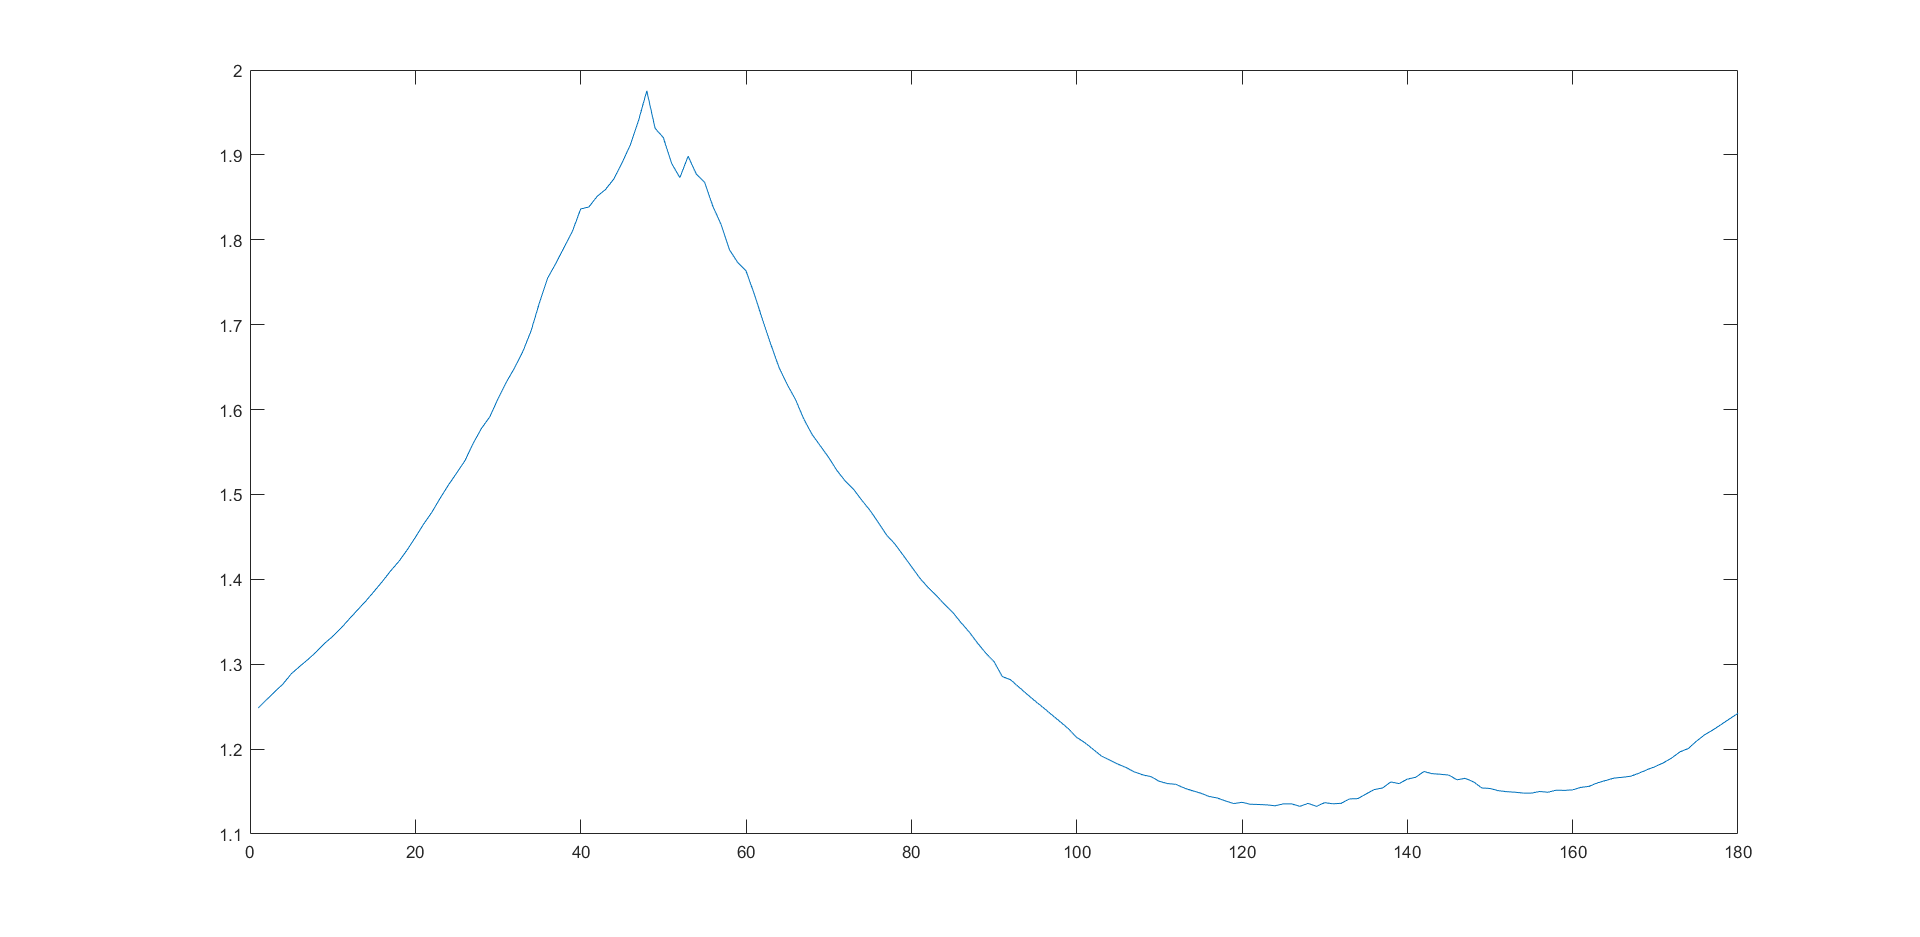
\includegraphics[width=0.7\linewidth]{JFMMrt3.png}
	\caption{Sample figure caption.}
	\label{fig:JFMMrt3jpg}
\end{figure}

The x-axis in the above figure represents rotation -90~90 degrees (the label in the above figure is wrong), and the y-axis is the result of radon transform.

\paragraph{technical details}

(a) Data flow

(1)Control flow

\begin{figure}
	\centering
	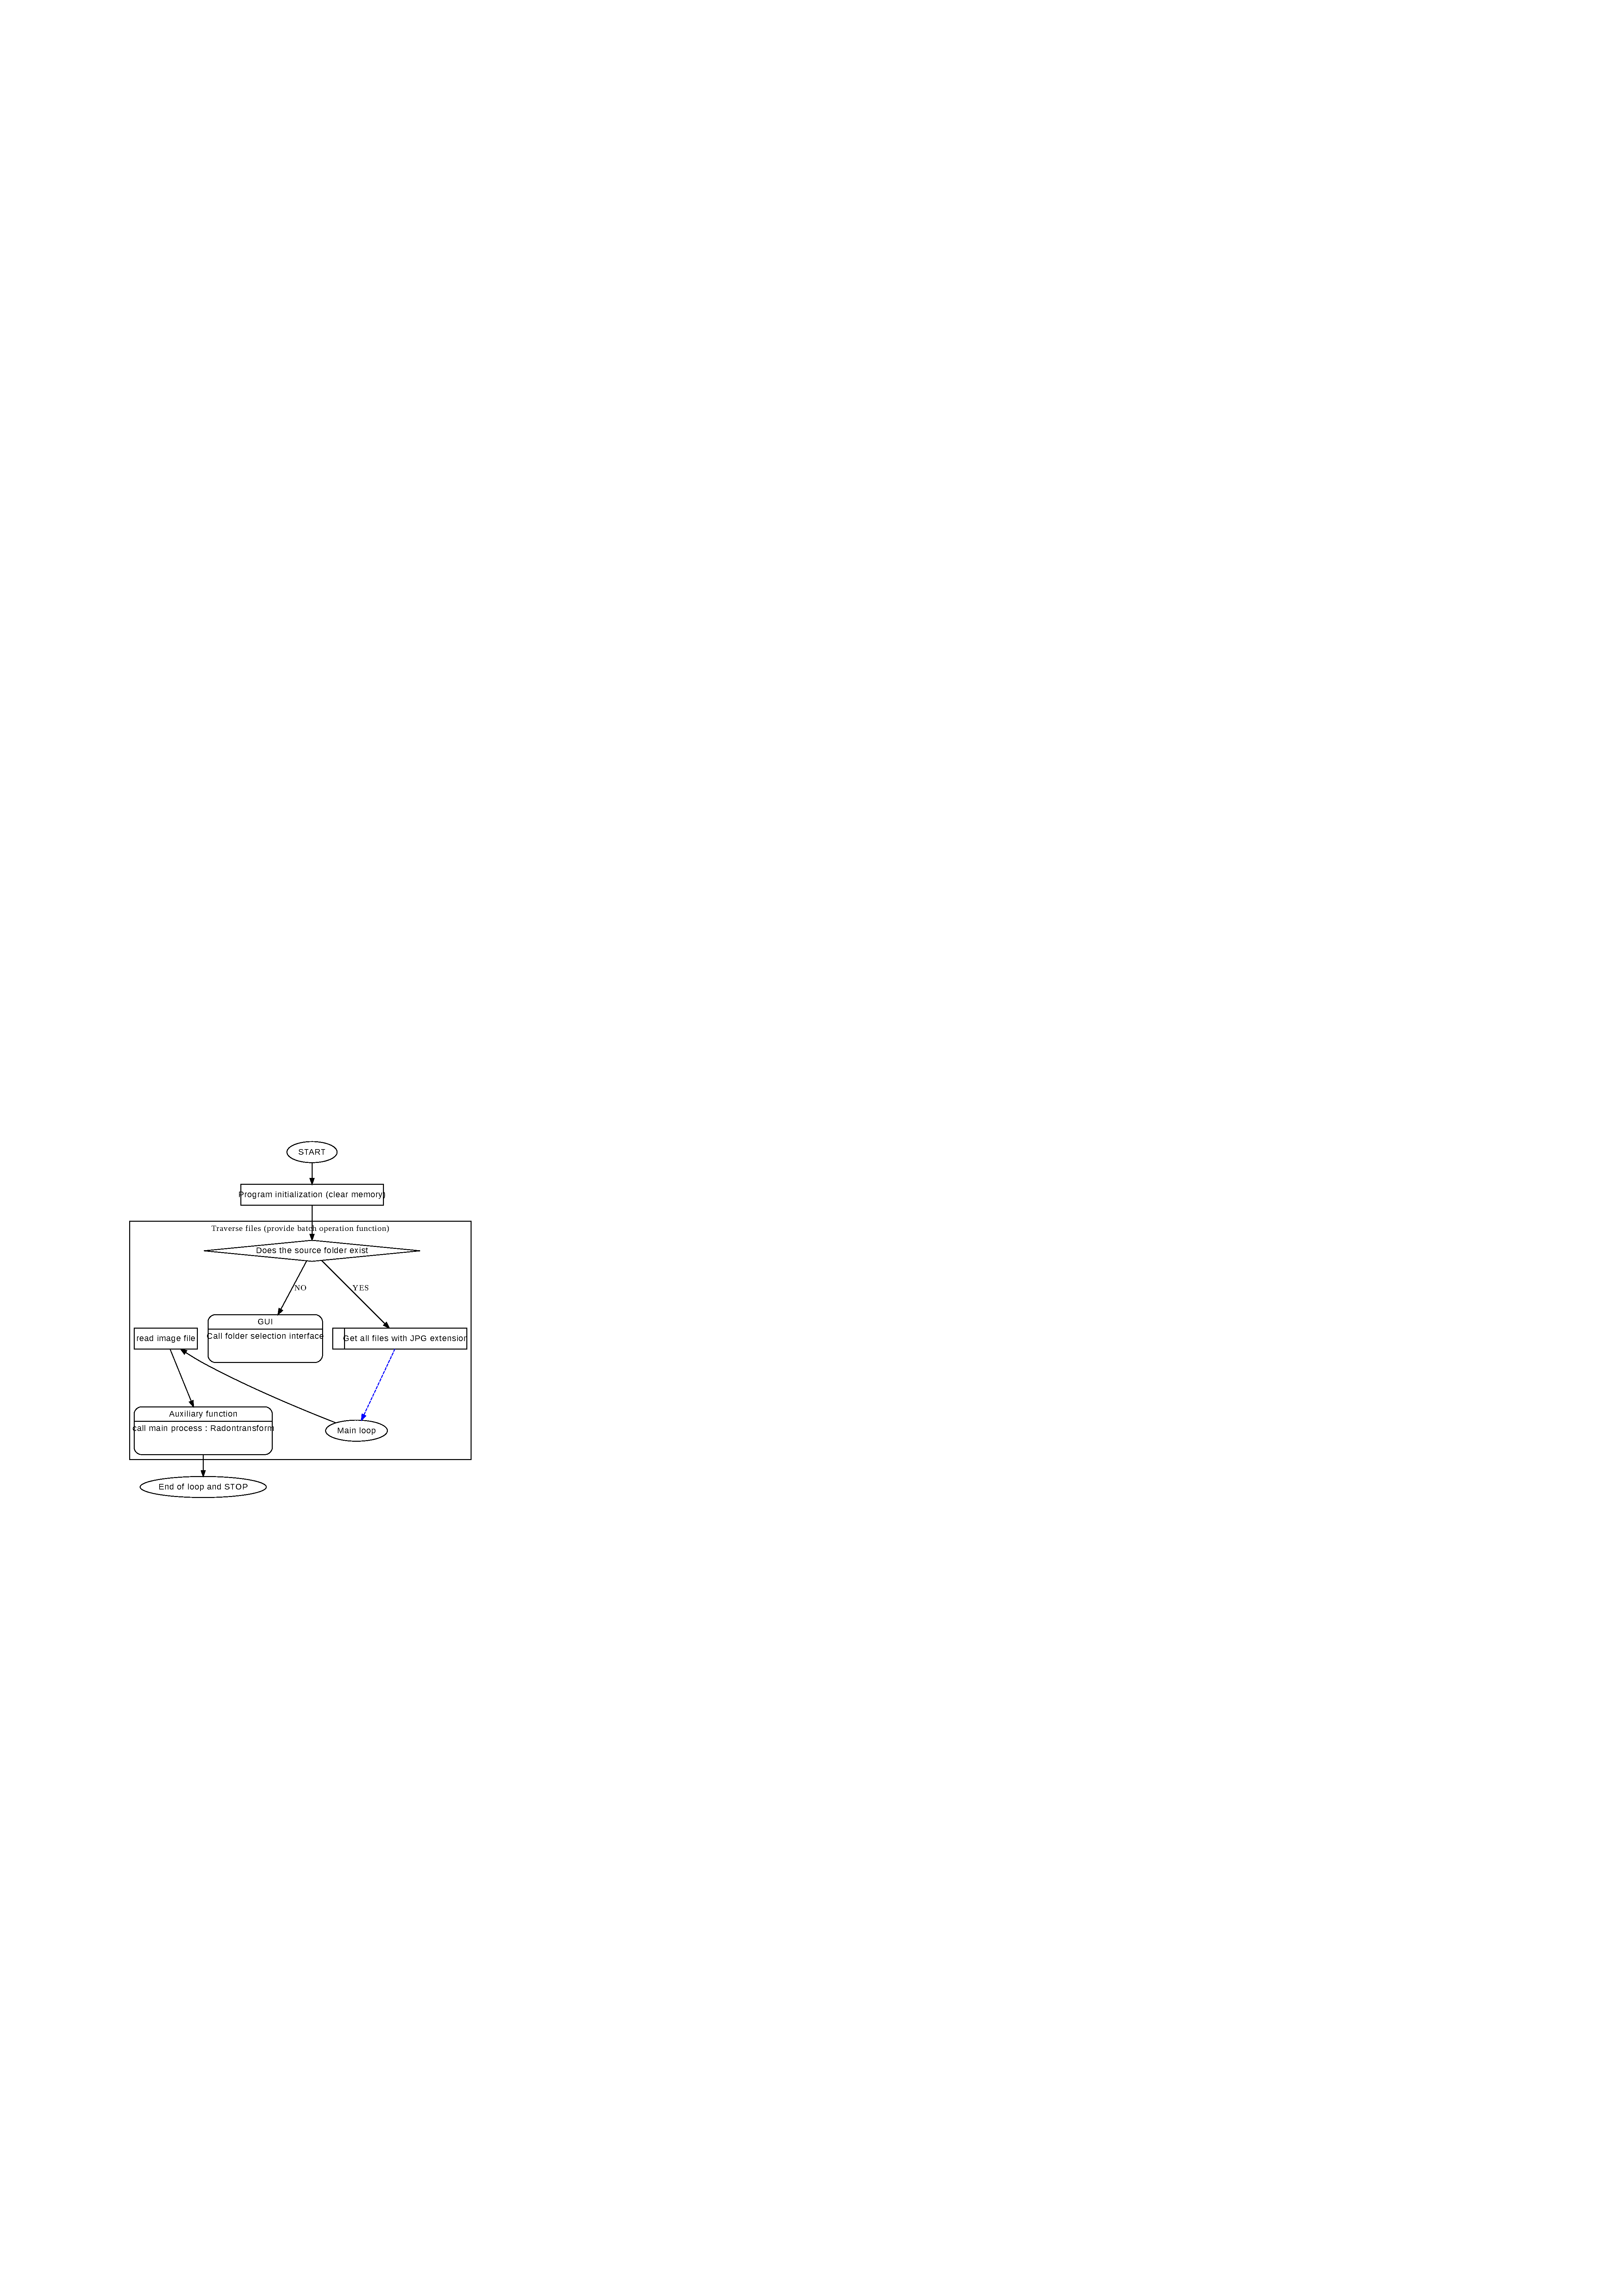
\includegraphics[width=0.7\linewidth]{f0.pdf}
	\caption{Sample figure caption.}
	\label{fig:f0pdf}
\end{figure}

(2)radon transformation

\begin{figure}
	\centering
	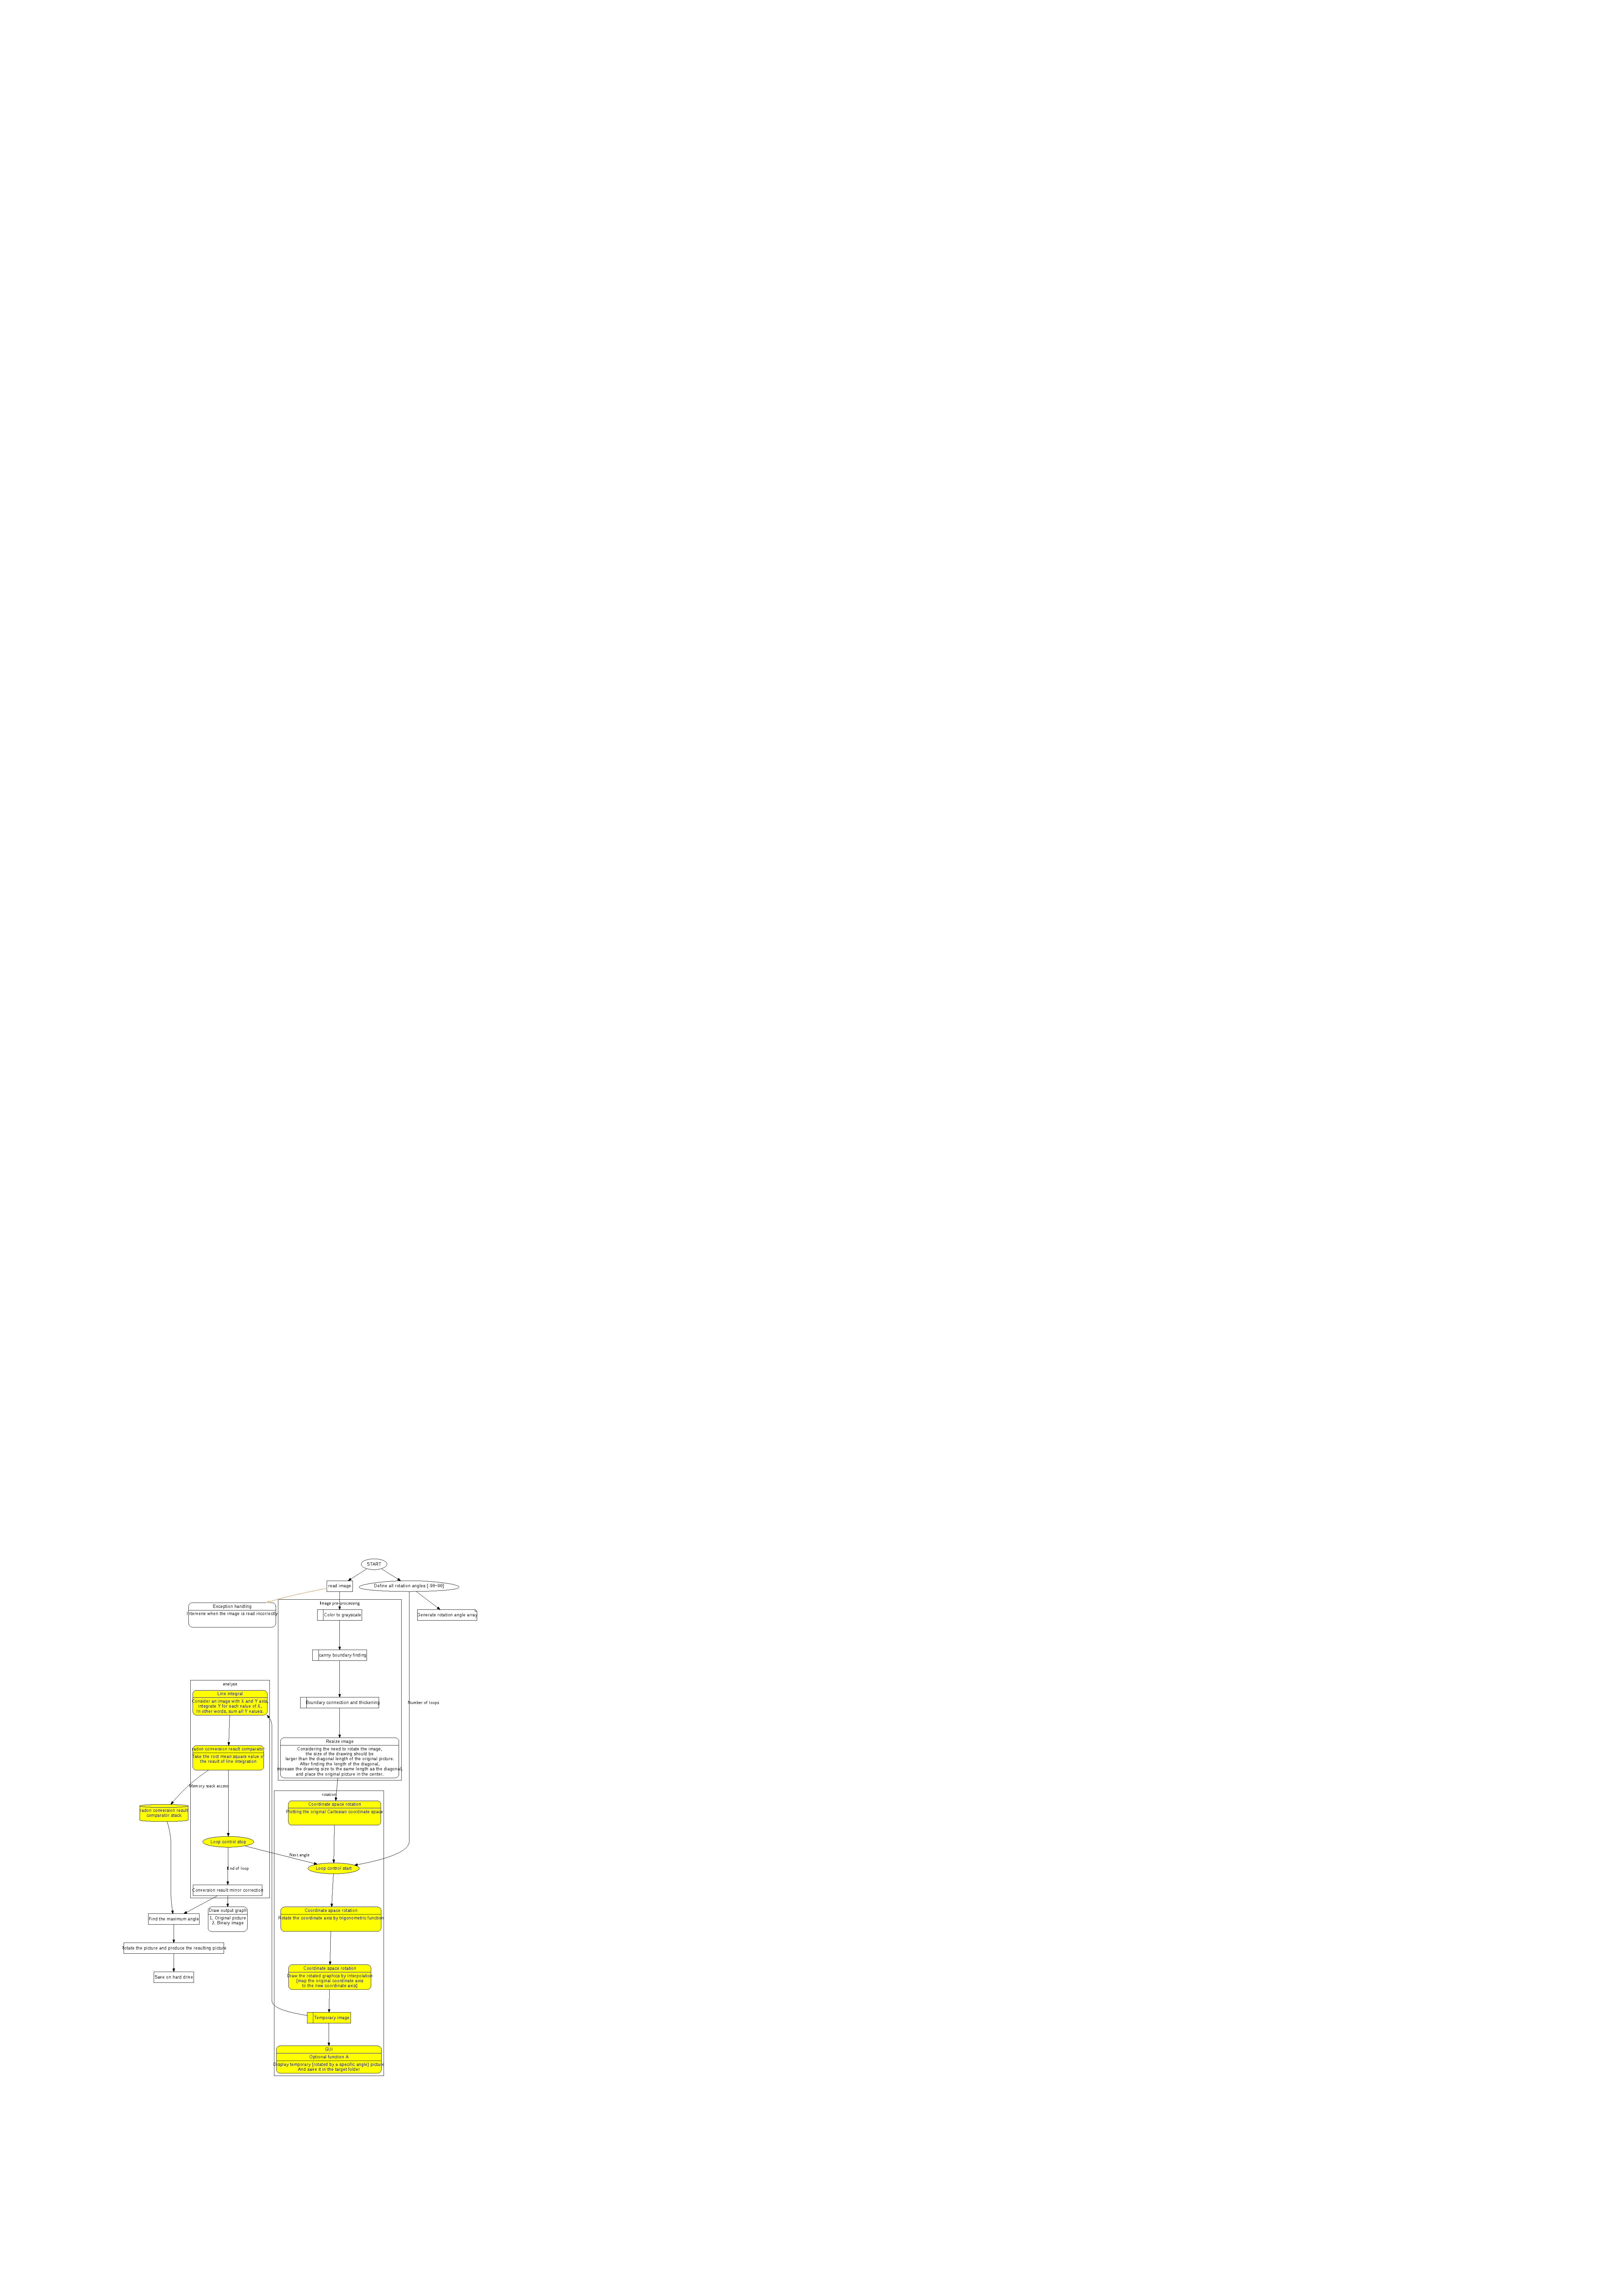
\includegraphics[width=0.7\linewidth]{f.pdf}
	\caption{Sample figure caption.}
	\label{fig:fpdf}
\end{figure}

%(b) Developer tools and debugging methods

%- Please keep the global variable "display and save results" true to provide all functions

%- Set the global variable "define print and save rotation angle coordinate conversion" to true, you can view the result of coordinate rotation by rotation angle (as shown in the figure below), but it will reduce the speed.

\begin{figure}
	\centering
	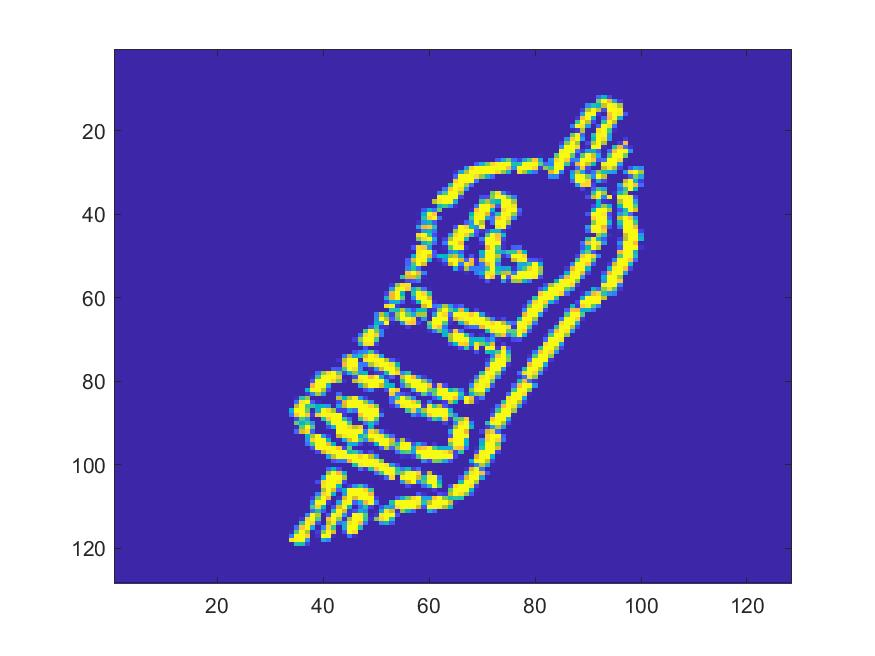
\includegraphics[width=0.7\linewidth]{6AdnkBj.jpg}
	\caption{Sample figure caption.}
	\label{fig:6AdnkBj}
\end{figure}

\paragraph{Highlights and features}

Matlab has a built-in radon transformation, but we did not use it, because the built-in function cannot be applied to the direction correction of the resistance. The reason is as follows: During line integration, the built-in function directly adds all the values in the line diameter directly, which leads to failure in the "line search" application, because discontinuous line segments (dashed lines) may have larger result values .
We use the weighting method. If the points are continuous, the result value will be increased, resulting in the "line finding" application becoming more effective.

\paragraph{Known defects}

At situations such as:
- The resolution of the picture is too low
- Too much noise
- Complex object texture
The above conditions will cause the boundary detection to output too much information, indirectly lead to too many internal entities in the input function of radon transformation.Resault to direction correction to fail at line integration stage.

%\paragraph{Test Modified Paragraph}

\subsubsection{Image recognition using traditional computer vision methods}
Treat the input color pictures according to the steps below to process the image:
1. Vague
2. Sotation
3. Find the critical value
We can analyze the geometric pattern distribution with different color channels. Unfortunately, because of the reflection relationship, one of the four ribbons will disappear to make this method feasible. Under practical conditions, using the action device to sampling the objects. In the case of turning on the flash, it will inevitably produce harmful reflection. If the flash is not opened, we will pick up in the case of insufficient light. Get the value of 0.
\begin{figure}
	\centering
	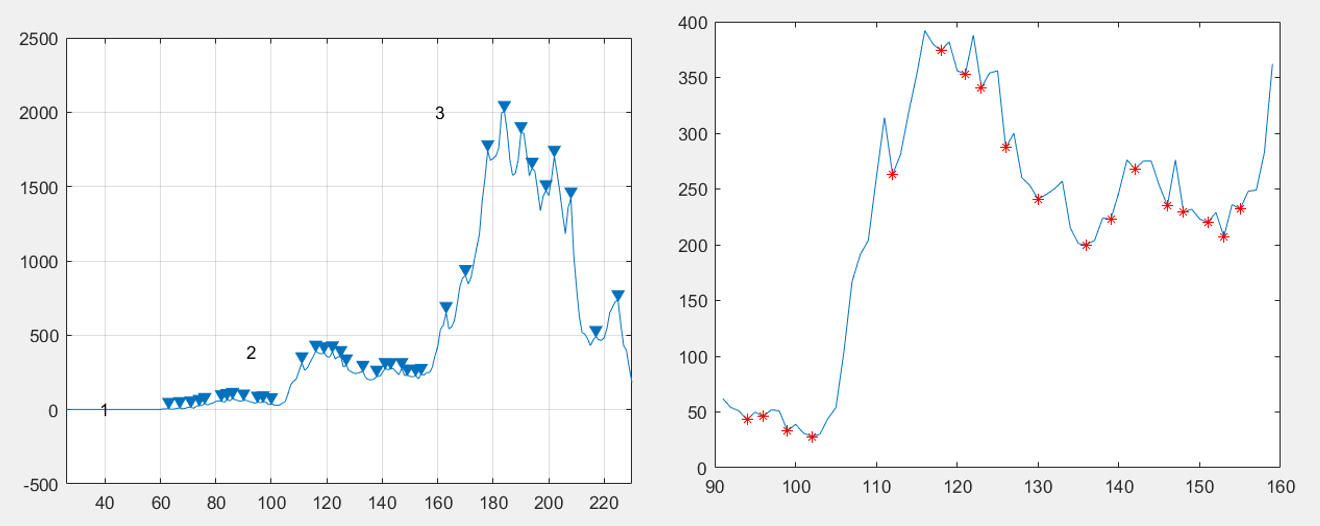
\includegraphics[width=0.7\linewidth]{tcv0.png}
	\caption{Sample figure caption.}
	\label{fig:tcv0}
\end{figure}
\begin{figure}
	\centering
	
\includegraphics[width=0.7\linewidth]{zz9.png}
	\caption{Sample figure caption.}
	\label{fig:zz9}
\end{figure}

\subsubsection{deep learning methods}
\subsection{System Design}
%\subsubsection{data collection}
%\subsubsection{image tag}

\subsubsection{Mobile device photo data generator}
\footnote{https://github.com/andythebreaker/camPdfHttpAndriod}
\paragraph{preamble}
To color correct as a cardboard
The camera must focus on the paper card, but in practice, the autofocus of the smartphone has the following problems

Speed varies by algorithm and hardware
Can't "autofocus" on very close objects
If there are people in the frame or unusual bright spots (such as reflections), the autofocus will defocus the specific
Native cameras don't know what a "color-specific card" or "resistance" is

\paragraph{problem analysis}

The above defects are all due to the autofocus algorithm of the native camera program, which is provided for general use.
If you need special functions, you need to write your own dynamic focus program or use manual focus

\paragraph{planning}

Control the camera with the base camera api
and take pictures
Make it focus on a given area of the program(like a resistor or a color card)

The above functions cannot be easily practiced with PWA
First test with the android system at hand

- Compose apk
- Implemented in java language

\paragraph{Overview of the current status of the android camera api}

- The old api `camera` has been largely abolished, and most devices with android 4.X are also disabled in hardware, only need to consider the new `camera2` api
- Given (the following quotes from google)
> The hardware implementation of `camera2` api of different manufacturers has different degrees of completeness, so start to develop a new generation of `cameraX` api

Most new android devices use `cameraX`
However, the latest version of `cameraX` was just updated on the 30th of last month (202106), and there is a lack of reference resources on the Internet. It depends on reading the original documents, and the development speed will be slightly later than the general situation.

- The above `cameraX` api is implemented based on the `camera2` api. Although it is more general and simple, if you need to use the lower-level functions, you may have to wait for the update of `cameraX` or call `camera2` directly
- The 202106 version of the above `cameraX` api only supports android 11 -> There is no hardware compatibility at all, there are not many devices on the market that can support android 11

\paragraph{Focus method}

\begin{figure}
	\centering
	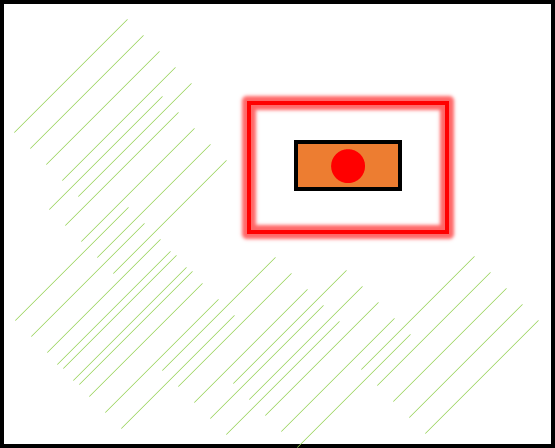
\includegraphics[width=0.7\linewidth]{oqKRMoT.png}
	\caption{Sample figure caption.}
	\label{fig:oqKRMoT}
\end{figure}

Pictured above

|Object|Description|
|--|--|
|Black Square|Camera Frame|
|Orange square|Target object (resistor or color card)|
|Red Dot|Focus Point (Zero Area)|
|Red Square|Focus Range|
|green lines|other irrelevant objects|

\paragraph{Action description}

Given a camera image, if you want to focus on an object, you can use the equation to specify the coordinates (or even the range) to achieve focus
\paragraph{advantages and disadvantages}

-The above-mentioned method of focusing on the 2D plane, not directly given the focusing distance (value), which leads to slow speed. You need to go through the "clear-blur" loop.
-It can also be called directly `camera2`api; but it seems to conflict with the function of the` camerax`api AF, and this problem has not been ruled out yet

\paragraph{Picture adjustment}

The same API also provides automatic adjustment of exposure and saturation. The method has been implemented at the top code.
\subsubsection{color correction}
For the errors of environmental light sources, such as: sunlight lamp tube color temperature is too cold or sunlight is transmitted to heat over heat ... When artificial labeling information, we can use manual or automatic ways to adjust the color bias. After drawing the distribution map first, we can first draw the distribution map. We can help make the distributed map back to normal
\begin{figure}
	\centering
	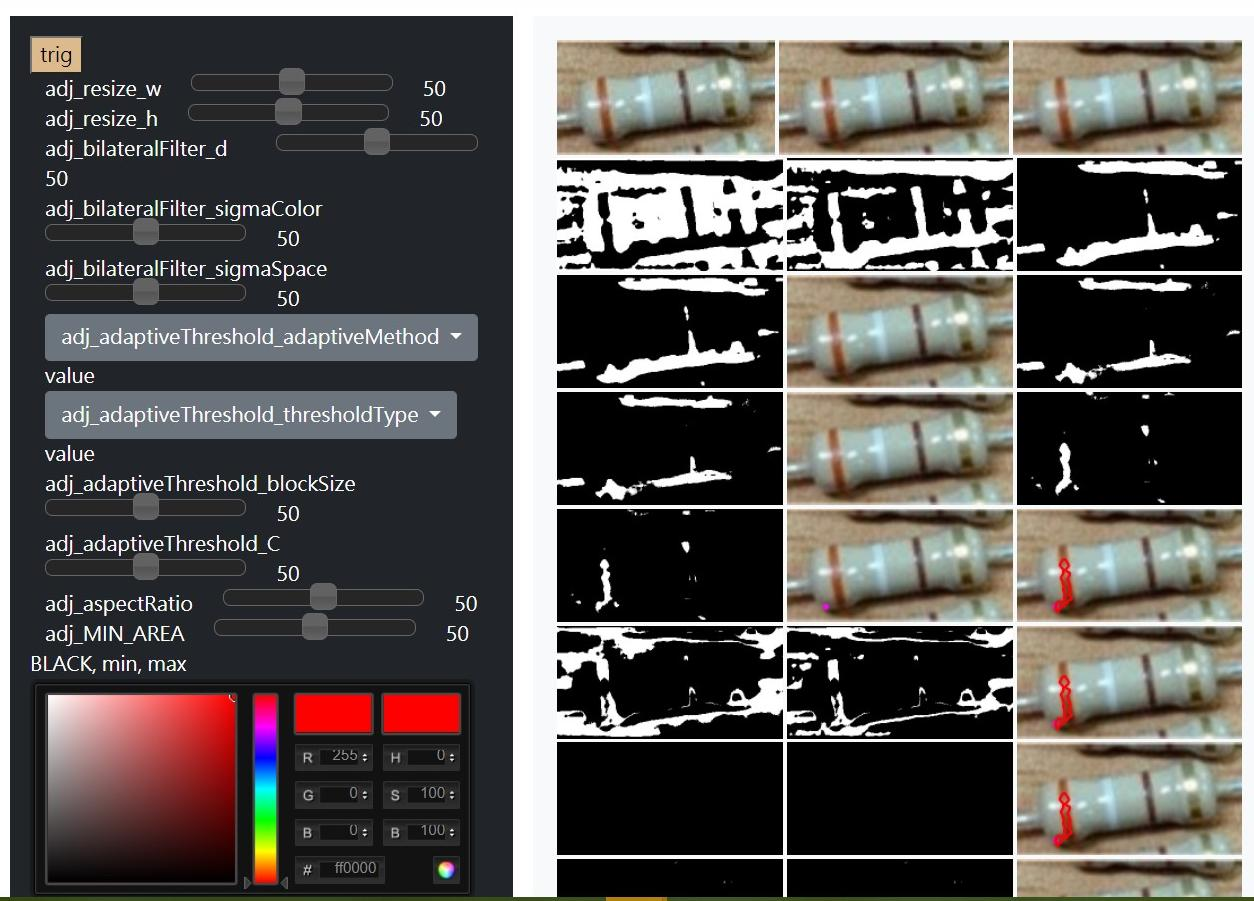
\includegraphics[width=0.7\linewidth]{CsXuTh9.jpg}
	\caption{Sample figure caption.}
	\label{fig:CsXuTh9}
\end{figure}

Direct diagram-> YOLO prediction-> manual ride-> again prediction-> get a positive resistance

Bilateral filter (Bilateral Filter)-> (RGB-> HSR (hue, saturation, brightness))-> [Adaptive dual-duty]-> reverse-> color segmentation screen-> get outline-> get obtained A range of large and wide length and width ratio
\subsubsection{Data collection}

\paragraph{Data curation and visualization}
\footnote{https://github.com/andythebreaker/picture\_set\_to\_slides\_converter}
picture set to slides converter
batch picture slideshow production

os
windows Tested in windows10.

Software function
Add the pictures in a folder to the presentation file one by one

Given some pictures (jpg), all installed in a folder.
Given a directory where output files can be placed.
The program will generate a presentation file (pptx) with all pictures.
Please note that the format of the image file name is strict.
The picture size will not be changed if the picture size is smaller than the size of the slide, otherwise it will be adjusted to fit the size of the slide.
The user can input the length and width centimeters of the target slide.

\begin{figure}
	\centering
	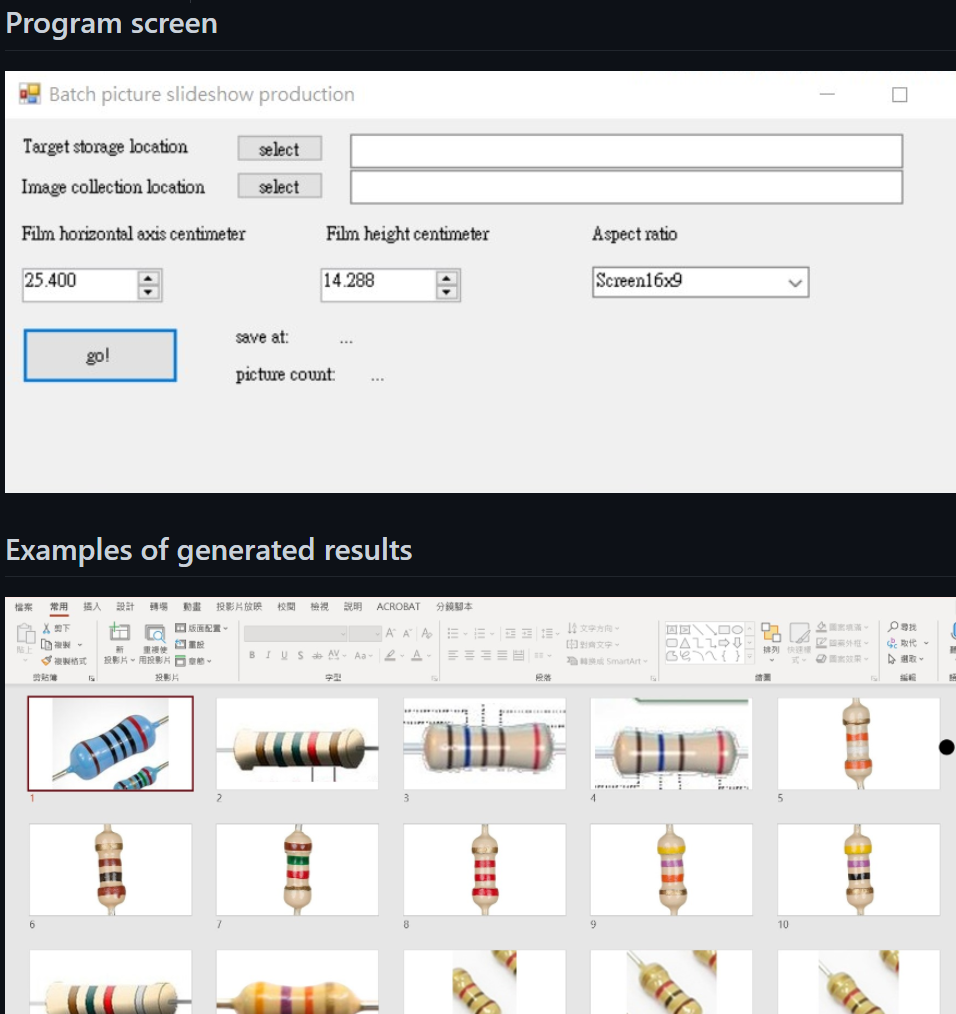
\includegraphics[width=0.7\linewidth]{SIj7pfq.png}
	\caption{Sample figure caption.}
	\label{fig:SIj7pfq}
\end{figure}
\paragraph{Database build}

\subsubsection{Transfer Learning}

\subsubsection{data augmentation}

\section{Experimental results}


\subsection{traditional computer vision methods}
\subsection{Using the YOLO Kit}
\subsection{attention model}
\subsection{WPA Marginal Operations}
\subsection{Mobile device real-time streaming}


\section{conclusion}
3. Thematic implementation plan
(1) Progress Gantt Chart
Please refer to the description below for the work code.
Description of work code:
1. Stage 1 (topic setting stage)
(1) Familiar with machine learning knowledge
(2) Literature search
(3) Find feasible research objectives
(4) Literature review
(5) Feasibility analysis
(6) Experimental environment setup (GCP)
(7) Experimental environment setup (Local GPU workstation)
(8) Manual data collection
(9) Manual data labeling
2. Phase 2 (basic function construction)
(1) True and false identification training
(2) Image recognition using yoloV5
(3) Fine-tuning
(4) Image classification task
3. Stage 3 (Accuracy Optimization)
(1) Color correction
(2) Image normalization using OpenCV
(3) Numerical identification using OpenCV
(4) Analysis and removal of divergent training data
(5) Auto data collection (Data crawling)
(6) Auto data labeling (cvat)
(7) Color correction optimization
(8) Image normalization optimization
(9) Numerical identification optimization
4. Stage 4 (performance optimization)
(1) Blur frame removal
(2) Optimization for video (continuous dynamic frames)
(3) Real-time recognition optimization
(4) Actual environment test
5. Phase 5 (Application Packaging)
(1) TensorFlow.js Web application building
(2) Model conversion
(3) Website back-end server setup
(4) User interface drawing
(5) Build front-end UI

%% \section{Headings: first level}
%% \label{sec:headings}
%% 
%% \lipsum[4] See Section \ref{sec:headings}.
%% 
%% \subsection{Headings: second level}
%% \lipsum[5]
%% \begin{equation}
%% 	\xi _{ij}(t)=P(x_{t}=i,x_{t+1}=j|y,v,w;\theta)= {\frac {\alpha _{i}(t)a^{w_t}_{ij}\beta _{j}(t+1)b^{v_{t+1}}_{j}(y_{t+1})}{\sum _{i=1}^{N} \sum _{j=1}^{N} \alpha _{i}(t)a^{w_t}_{ij}\beta _{j}(t+1)b^{v_{t+1}}_{j}(y_{t+1})}}
%% \end{equation}
%% 
%% \subsubsection{Headings: third level}
%% \lipsum[6]
%% 
%% \paragraph{Paragraph}
%% \lipsum[7]



\section{Examples of citations, figures, tables, references}
\label{sec:others}

\subsection{Citations}
Citations use \verb+natbib+. The documentation may be found at
\begin{center}
	\url{http://mirrors.ctan.org/macros/latex/contrib/natbib/natnotes.pdf}
\end{center}

Here is an example usage of the two main commands (\verb+citet+ and \verb+citep+): Some people thought a thing \citep{kour2014real, hadash2018estimate} but other people thought something else \citep{kour2014fast}. Many people have speculated that if we knew exactly why \citet{kour2014fast} thought this\dots

\subsection{Figures}
\lipsum[10]
See Figure \ref{fig:fig1}. Here is how you add footnotes. \footnote{Sample of the first footnote.}
\lipsum[11]

\begin{figure}
	\centering
	\fbox{\rule[-.5cm]{4cm}{4cm} \rule[-.5cm]{4cm}{0cm}}
	\caption{Sample figure caption.}
	\label{fig:fig1}
\end{figure}

\subsection{Tables}
See awesome Table~\ref{tab:table}.

The documentation for \verb+booktabs+ (`Publication quality tables in LaTeX') is available from:
\begin{center}
	\url{https://www.ctan.org/pkg/booktabs}
\end{center}


\begin{table}
	\caption{Sample table title}
	\centering
	\begin{tabular}{lll}
		\toprule
		\multicolumn{2}{c}{Part}                   \\
		\cmidrule(r){1-2}
		Name     & Description     & Size ($\mu$m) \\
		\midrule
		Dendrite & Input terminal  & $\sim$100     \\
		Axon     & Output terminal & $\sim$10      \\
		Soma     & Cell body       & up to $10^6$  \\
		\bottomrule
	\end{tabular}
	\label{tab:table}
\end{table}

\subsection{Lists}
\begin{itemize}
	\item Lorem ipsum dolor sit amet
	\item consectetur adipiscing elit.
	\item Aliquam dignissim blandit est, in dictum tortor gravida eget. In ac rutrum magna.
\end{itemize}


\bibliographystyle{unsrtnat}
\bibliography{references}  %%% Uncomment this line and comment out the ``thebibliography'' section below to use the external .bib file (using bibtex) .


%%% Uncomment this section and comment out the \bibliography{references} line above to use inline references.
% \begin{thebibliography}{1}

% 	\bibitem{kour2014real}
% 	George Kour and Raid Saabne.
% 	\newblock Real-time segmentation of on-line handwritten arabic script.
% 	\newblock In {\em Frontiers in Handwriting Recognition (ICFHR), 2014 14th
% 			International Conference on}, pages 417--422. IEEE, 2014.

% 	\bibitem{kour2014fast}
% 	George Kour and Raid Saabne.
% 	\newblock Fast classification of handwritten on-line arabic characters.
% 	\newblock In {\em Soft Computing and Pattern Recognition (SoCPaR), 2014 6th
% 			International Conference of}, pages 312--318. IEEE, 2014.

% 	\bibitem{hadash2018estimate}
% 	Guy Hadash, Einat Kermany, Boaz Carmeli, Ofer Lavi, George Kour, and Alon
% 	Jacovi.
% 	\newblock Estimate and replace: A novel approach to integrating deep neural
% 	networks with existing applications.
% 	\newblock {\em arXiv preprint arXiv:1804.09028}, 2018.

% \end{thebibliography}


\end{document}
